\documentclass[tikz,border=5pt]{standalone}
\usepackage{tikz}
\usepackage{graphicx}
\pagestyle{empty}
\begin{document}
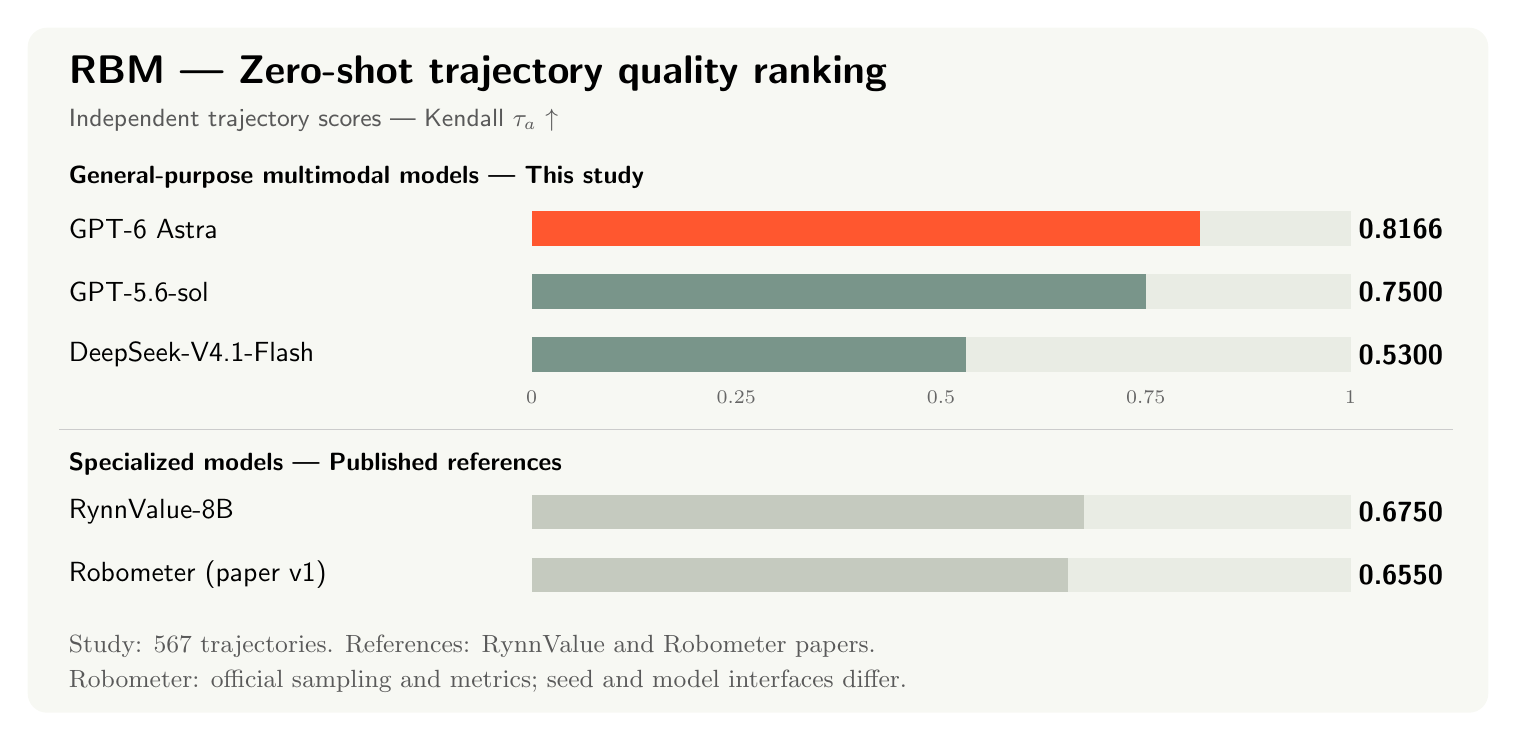
\begin{tikzpicture}[x=1cm,y=1cm,font=\sffamily]
\definecolor{cardbg}{HTML}{F7F8F3}
\definecolor{trackbg}{HTML}{E9ECE4}
\definecolor{mutedbar}{HTML}{C5CABF}
\definecolor{astrabar}{HTML}{FF572F}
\definecolor{iclbar}{HTML}{F4A082}
\definecolor{studybar}{HTML}{79958A}
\fill[cardbg,rounded corners=7pt] (-.4,2) rectangle (18.15,-6.7);
\node[anchor=west,font=\sffamily\bfseries\Large] at (0,1.42) {RBM | Zero-shot trajectory quality ranking};
\node[anchor=west,font=\sffamily\small,text=black!65] at (0,.82) {Independent trajectory scores | Kendall $\tau_a$ $\uparrow$};
\node[anchor=west,font=\sffamily\bfseries\small] at (0,.1) {General-purpose multimodal models | This study};
\node[anchor=west,font=\sffamily] at (0,-0.55) {GPT-6 Astra};
\fill[trackbg] (6,-0.77) rectangle (16.4,-0.33000000000000007);
\fill[astrabar] (6,-0.77) rectangle (14.492640,-0.33000000000000007);
\node[anchor=east,font=\sffamily\bfseries] at (17.7,-0.55) {0.8166};
\node[anchor=west,font=\sffamily] at (0,-1.35) {GPT-5.6-sol};
\fill[trackbg] (6,-1.57) rectangle (16.4,-1.1300000000000001);
\fill[studybar] (6,-1.57) rectangle (13.800000,-1.1300000000000001);
\node[anchor=east,font=\sffamily\bfseries] at (17.7,-1.35) {0.7500};
\node[anchor=west,font=\sffamily] at (0,-2.15) {DeepSeek-V4.1-Flash};
\fill[trackbg] (6,-2.37) rectangle (16.4,-1.93);
\fill[studybar] (6,-2.37) rectangle (11.512000,-1.93);
\node[anchor=east,font=\sffamily\bfseries] at (17.7,-2.15) {0.5300};
\node[text=black!60,font=\scriptsize] at (6.0,-2.7) {0};
\node[text=black!60,font=\scriptsize] at (8.6,-2.7) {0.25};
\node[text=black!60,font=\scriptsize] at (11.2,-2.7) {0.5};
\node[text=black!60,font=\scriptsize] at (13.8,-2.7) {0.75};
\node[text=black!60,font=\scriptsize] at (16.4,-2.7) {1};
\draw[black!20] (0,-3.1) -- (17.7,-3.1);
\node[anchor=west,font=\sffamily\bfseries\small] at (0,-3.55) {Specialized models | Published references};
\node[anchor=west,font=\sffamily] at (0,-4.15) {RynnValue-8B};
\fill[trackbg] (6,-4.37) rectangle (16.4,-3.93);
\fill[mutedbar] (6,-4.37) rectangle (13.020000,-3.93);
\node[anchor=east,font=\sffamily\bfseries] at (17.7,-4.15) {0.6750};
\node[anchor=west,font=\sffamily] at (0,-4.95) {Robometer (paper v1)};
\fill[trackbg] (6,-5.17) rectangle (16.4,-4.73);
\fill[mutedbar] (6,-5.17) rectangle (12.812000,-4.73);
\node[anchor=east,font=\sffamily\bfseries] at (17.7,-4.95) {0.6550};
\node[anchor=west,text=black!65,font=\small] at (0,-5.85) {Study: 567 trajectories. References: RynnValue and Robometer papers.};
\node[anchor=west,text=black!65,font=\small] at (0,-6.3) {Robometer: official sampling and metrics; seed and model interfaces differ.};
\end{tikzpicture}
\end{document}
